\documentclass[12pt,a4paper]{article}

\usepackage[T1]{fontenc}
\usepackage{amsmath, amssymb, amsfonts}
\usepackage[magyar]{babel}
\usepackage[utf8]{inputenc}
\usepackage{graphicx}
\usepackage{graphics}
\usepackage{mathtools}
\usepackage{epsfig}
\usepackage{epstopdf}
\usepackage{cite}
\usepackage{caption}
\usepackage{hyperref}
\usepackage[bottom=4cm]{geometry}
%\geometry{a4paper, portrait, margin=1in}

\title{\huge{Korszerű vizsgálati módszerek labor jegyzőkönyv}\\ \vspace{20pt}
\textbf{Magspektroszkópiai vizsgálatok} \\}

\author{\Large{\textsc{Csörnyei Géza}} \vspace{10pt}\\
	\textrm{Eötvös Loránd Tudományegyetem}\\
	\textrm{Fizika BSc III. évfolyam}
	}
\date{}
%\lhead{}
\begin{document}
\addtolength{\voffset}{-1.5cm}
\addtolength{\textheight}{1.5cm}
\begin{titlepage}
\maketitle

\begin{figure}[!htb]
\centering
  
\includegraphics[scale=0.6]{eltecimer.jpg}
\end{figure}

\hfil \Large{'C' mérőcsoport}\hfil  \\
\vspace*{2pt}
\hfil \Large{\emph{Mérés dátuma:} 2018.03.22.}\hfil \\
\vspace*{2pt}
\hfil \Large{\emph{Mérés vezetője:} Pávó Gyula}\hfil \\
\vspace*{2pt}
\hfil \hspace*{45pt} \Large{\emph{Mérőtársak:} Szigeti Balázs, Szűcs Bálint}\hfil
\thispagestyle{empty}
\end{titlepage}


\section{Bevezetés}

A magfizikai kutatásokban és az izotóptechnikában fontos szerepet játszanak a különböző sugárzások. Ezek detektálásával és az energiaspektrumaik felvételével az adott kísérlet szempontjából lényeges információkhoz lehet jutni. A három féle radioaktív sugárzás közül (alfa,béta,gamma), a béta és a gamma sugárzások vizsgálata a legfontosabb. A béta sugárzás elektronokból vagy pozitronokból áll és töltött részecskenyalábhoz híven vastagabb anyag akár több réteg papír is már elnyeli. A gamma sugárzás nagy energiájú semleges fotonokból áll így ezeket nehéz leárnyékolni. Az utóbb említett két különböző sugárzás, tulajdonságainál fogva eltérő detektálási módszert, eltérő detektort kíván. Jelen mérésünkben energia szelektív számlálótípusú szcintillációs számlálót és félvezető detektort alklamazunk az energia spektrumok felvételére.\newline
Jelen mérésünk célja, hogy megismerkedjünk a gamma és béta spektroszkópia módszereivel, kísérleti analízisével.
\newpage
\subsection{Feladat kiosztás}
\begin{itemize}
\item Csörnyei Géza : Gamma spektroszkópia
\item Szigeti Balázs : Béta spektroszkópia
\item Szűcs Bálint : Szöveges kidolgozás
\end{itemize}
\subsection{Gamma spektroszkópiához használt mérőlánc beállítása}
\begin{itemize}
\item Detektor: 
Gamma gyártmányú, ND-305/g típusú, 80049 gyári számú mérõfej, gamma szcintillátorral.
\item Nagyfesz: NB 215.2 1000 V
\item Mérõlánc:
A rack jobb szélén lévõ, Canberra gyártmányú, 2012 típusú spektroszkópiaia erõsítõ; 
negatív bemeneti polaritás, (4*6,0) erõsítés, unip. kimenet.
\item Analizátor:
Atomki gyártmányú, PalmtopMCA típusú analizátor; 
512 csatorna.
\end{itemize}
\subsection{HPG mérőlánc beállítása}
A Debrecenből - javításként kapott - PalmtopMCA mérés beállítása: \begin{itemize}
\item Tc 241: 
10*7,0 erősítés, + bemenet, P/z állás, unipol kimenet. Így a teteje 3,78 MeV
\end{itemize}
A (korábbi) átállítás időpontja ismeretlen.
\begin{itemize}
\item 935 ADC: 
10 V, inp. bemenet; 
\begin{itemize}
\item néha vannak 6 V-os, "levágott fejű" impulzusok
\item threshold: 40 ch
\item peaking time: 13 us (20->13); pocsék p/z-vel
\end{itemize}
\end{itemize}
\subsection{Béta spektroszkópia mérőlánc beállításai}
\begin{itemize}
\item Detektor
Gamma gyártmányú, ND-319/g típusú, 92020 gyári számú mérõfej, béta szcintillátorral.
\item Mérõlánc
1/10-es frekvenciakompenzált feszültségosztó;
Canberra gyártmányú, 2012 típusú spektroszkópiaia erõsítõ; 
negatív bemeneti polaritás, (8*6,0) erõsítés, unip. kimenet.
\item Analizátor
Atomki gyártmányú, PalmtopMCA analizátor; 
10 V-os bemenet, 512 csatorna
\end{itemize}
\newpage
\section{Gamma spektroszkópia}
\subsection{Szcintillációs detektor}
\hspace*{10pt} A gamma spektroszkópiai vizsgálatainkat a szcintillációs detektor kalibrálásával kezdtük. Erre azért volt szükség, mert a spektrumokat sokcsatornás analizátor segítségével vettük fel, melynek csatornáihoz a kalibráció segítségével tudtunk energiatartományokat párosítani. A kalibráció során a spektrumokban látható egyes ismert energiájú csúcsokat Gauss-görbével illesztettem, melynek illesztéshez használt alakja:
$$f(x)=A\cdot e^{-\frac{(x-\mu)^2}{2\cdot \sigma ^2}} + c  .$$
A $c$ tagot a kontinuumszint figyelembevétele miatt kellett hozzáadnunk a görbéhez. A mérés jellege miatt a kontinuum exponenciális függvénnyel történő figyelembevétele lett volna a legmegfelelőbb, azonban az így behozott exponenciális tag megnehezítette volna az illesztési eljárást. Emiatt a csúcsok környezetében a kontinuumot közelítőleg lineárisnak tételeztem fel, mellyel becslésem szerint a statisztikus (Poisson) hibánál jóval kisebb hibával terheltem a kiértékelést. A kalibrációhoz az illesztett görbék közepét (átlagát) kellett vennünk, és kellett összevetnünk a csúcsok ismert energiaértékeivel. A vizsgálat során felvett spektrumok at \ref{fig:1} ., míg az illesztések az \ref{fig:2} . és a \ref{fig:3} . ábrákon láthatók.\\
\begin{figure}[!h]
\centering
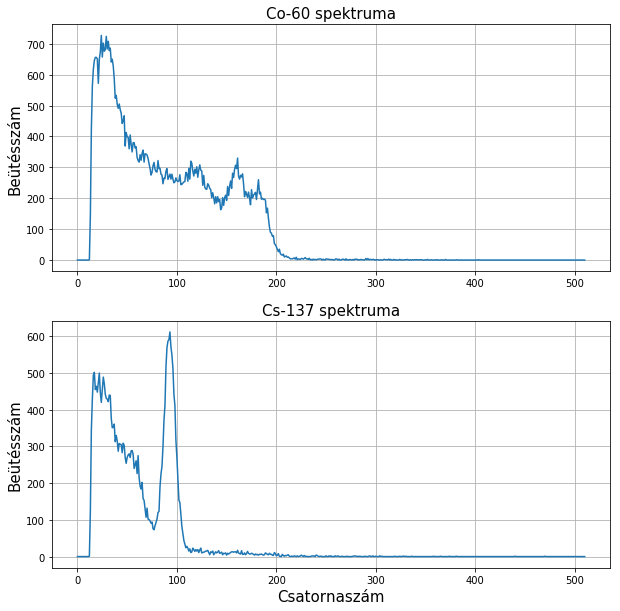
\includegraphics[scale=0.53]{szc_spekt}
\caption{A szcintillációs detektorral 120 s hosszú méréssel kapott spektrumok}
\label{fig:1}
\end{figure}
\newpage
\begin{figure}[!h]
\hspace*{-0.75cm}
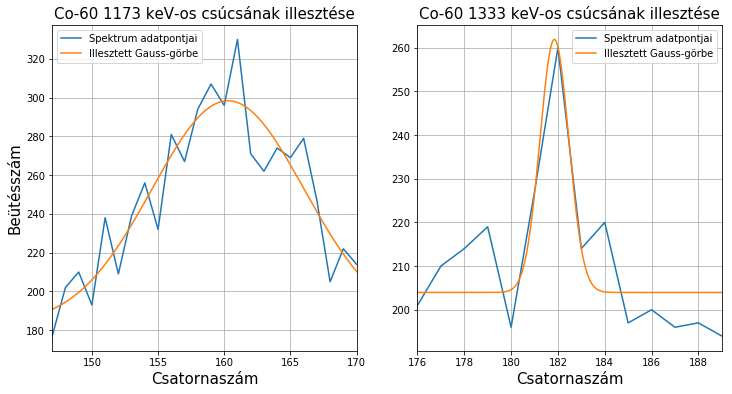
\includegraphics[scale=0.53]{Cob_figs}
\caption{A kobalt spektrumában látható első (1173 keV) és második (1333) csúcs illesztése}
\label{fig:2}
\end{figure}

Az illesztési paraméterek a fenti függvényalaknak megfelelő jelölésekkel:
\begin{table}[!h]
\begin{center}
\begin{tabular}{|c|c||c|}
\hline
Energia & 1173 keV & 1333 keV \\ 
\hline
$A$ & $115.619 \pm 18.067$ & $57.927 \pm 11.078$\\
\hline
$\mu$ & $160.286 \pm 0.400$ & $181.849 \pm 0.171$\\
\hline
$\sigma$ & $5.740 \pm 1.090$ & $0.616 \pm 0.139$ \\
\hline
$c$ & $182.754 \pm 19.411$ & $203.965 \pm 3.019$\\
\hline
\end{tabular}
\caption{A kobalt spektrumában látható csúcsok illesztési paraméterei}
\end{center}
\end{table}

\newpage

\begin{figure}[!h]
\centering
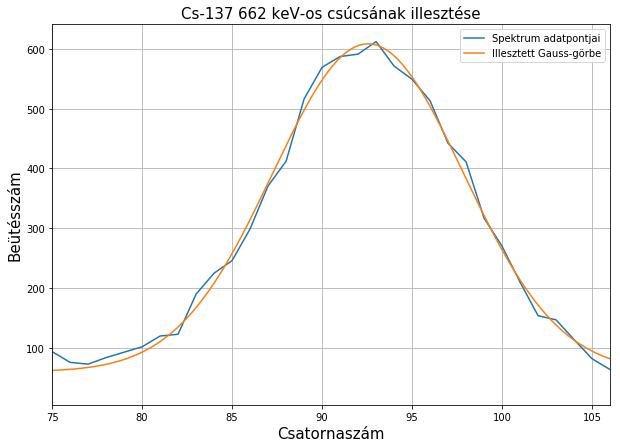
\includegraphics[scale=0.60]{Cs137_1csucs}
\caption{A cézium spektrumában látható csúcs (662 keV) illesztése}
\label{fig:3}
\end{figure}
Az illesztési paraméterek:
\begin{table}[!h]
\begin{center}
\begin{tabular}{|c|c|}
\hline
Energia & 662 keV \\ 
\hline
$A$ & $547.931 \pm 8.419$\\
\hline
$\mu$ & $92.557 \pm 0.076$\\
\hline
$\sigma$ & $5.291 \pm 0.117$\\
\hline
$c$ & $60.276 \pm 6.702$\\
\hline
\end{tabular}
\caption{A cézium spektrumában látható csúcs illesztési paraméterei}
\end{center}
\end{table}

\newpage
A kalibráció szempontjából fontos mennyiség számunkra a csúcsok helye, azaz a csatornaszám, melyen az illesztett Gauss-görbe átlaga van. Ezen értékek, valamint a csúcsokhoz tartozó energiaértékek ismeretében el tudjuk végezni a kalibrálást egyenesillesztés képében, mely a \ref{fig:4} . ábrán látható.

\begin{figure}[!h]
\centering
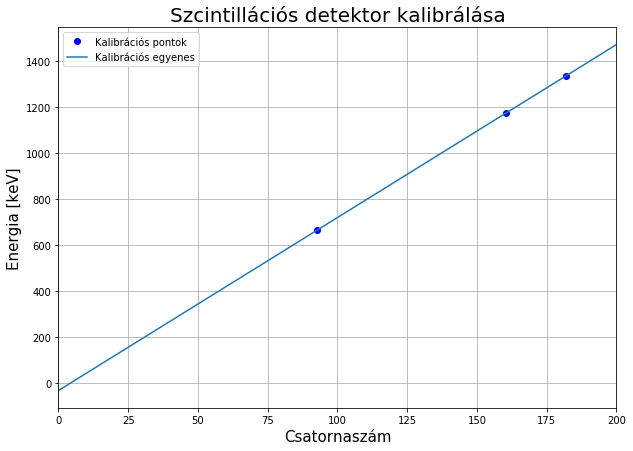
\includegraphics[scale=0.60]{Szcint_kalib}
\caption{A szcintillációs detektor kalibrálásához készített egyenesillesztés}
\label{fig:4}
\end{figure}

Az illesztett egyenes egyenlete:
$$ E(x) = 7.522 \cdot x - 33.903 ,$$
ahol $x$ a csatornaszámot jelöli, valamint mind a két oldal keV egységekben értendő.\\
\hspace*{10pt} A kalibráció elvégzése után lehetőségünk nyílt a detektor felbontóképességének meghatározására. Ehhez a $^{60}$Co 1333 keV-os csúcsának félértékszélességét számítottuk ki, ugyanis ez jól jellemezte a detektor felbontóképességét. Ennek oka, hogy csúcs mindössze egyetlen csatornában mért kiugró beütésszám értékként jelent meg, a szomszédos csatornákban már a kontinuumszinthez hasonló értékeket lehetett mérni. A félérték szélesség számításához az [1]-ben leírtaknak megfelelően lehet eljárni, azaz keV-ben mérve a félértékszélességet közelítőleg az 
$$ \Delta x = 2.36 \cdot \sigma $$
képlet határozza meg, ahol $\sigma$ az illesztett Gauss-görbe szórása. Ennek értelmében a fentebb említett mérés felhasználásával a mért félértékszélességre $ \Delta x = (10.934 \pm 2.475)$ keV adódik.\\
\newpage
A szcintillációs detektor segítségével felvettük egy NaCl (háttér) és egy KCl minta spektrumát is, majd meghatároztuk az ezekben vett $^{40}K$ intenzitás arányát. A felvett spektrumok a \ref{fig:5} . ábrán láthatók.
\begin{figure}[!h]
\centering
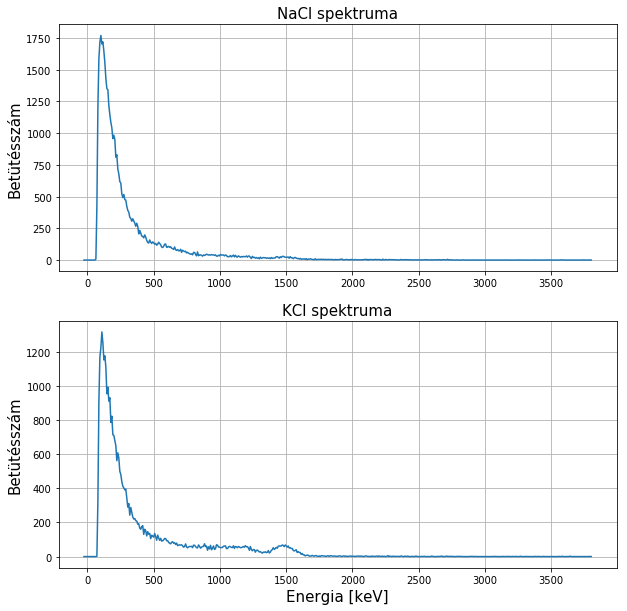
\includegraphics[scale=0.60]{Na-K_spek}
\caption{NaCl és KCl mintákkal felvett spektrumok}
\label{fig:5}
\end{figure}
\newline
A $^{40}$K-hez tartozó csúcsok és azok illesztései a két spektrum esetében a \ref{fig:6} . ábrán láthatók. Mivel a csúcs környékén a kontiunnum nem volt állandó értékkel közelíthető, ezért a csúcsok illesztése során a Gauss-görbét az alábbi módon egészítettük ki:
$$f(x)=A\cdot e^{-\frac{(x-\mu)^2}{2\cdot \sigma ^2}} + cx + b  .$$
A csúcsok intenzitásának arányánál az együtthatóikat vetettük össze, ez azonban nem egyezik meg az illesztés során használt $A$-val, a Gauss-görbe definíciójából adódóan. Ennek megfelelően
$$A=A^{*}\frac{1}{\sqrt{2\pi \sigma}},$$
ahol $A^{*}$ az általunk használni kívánt intenzitás (egyben beütésszám) érték.
\newpage
\begin{figure}[!h]
\centering
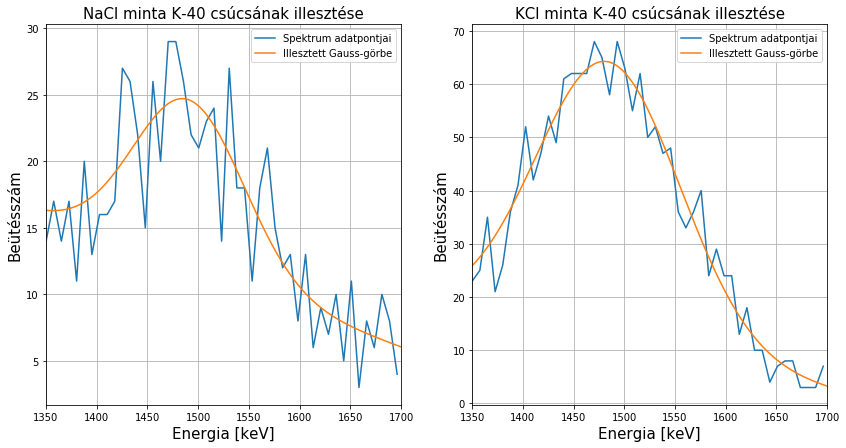
\includegraphics[scale=0.50]{K40_fits}
\caption{NaCl és KCl mintákkal mért $^{40}$K csúcsok és azok illesztései. A NaCl mintával végzett mérés 120 s-ig tartott, kétszer annyi ideig, míg a KCl mintával végzett mérés, így a kapott amplitúdó kétszeresével kell számolni a KCl minta esetében.}
\label{fig:6}
\end{figure}

Az illesztési paramétereket az alábbi táblázat tartalmazza:
\begin{table}[!h]
\begin{center}
\begin{tabular}{|c|c||c|}
\hline
- & NaCl minta & KCl minta \\
\hline
$A$ & $12.712 \pm 1.512$ & $52.755 \pm 2.545$ \\
\hline
$\mu$ [keV] & $1490.893 \pm 7.321$ & $1484.088 \pm 3.195$ \\ 
\hline
$\sigma$ [keV] & $54.592 \pm 9.233$ & $71.317 \pm 4.599$ \\
\hline
$c$ [1/keV] & $-0.028 \pm 0.006$ & $-0.040 \pm 0.010$ \\
\hline
$b$ & $53.731 \pm 9.405$ & $71.363 \pm 17.232$ \\
\hline
\end{tabular}
\caption{$^{40}$K csúcsokra vonatkozó illesztési paraméterek}
\end{center}
\end{table}
\newline
A fentiek alapján a két csúcs intenzitásának, így amplitúdóinak arányát az alábbi módon lehet számolni:
$$\frac{1}{2}\frac{A^{*}_{\textrm{NaCl}}}{A^{*}_{\textrm{KCl}}}=
\frac{A_{\textrm{NaCl}}}{A_{\textrm{KCl}}}\cdot  \frac{\sigma_{\textrm{NaCl}}}{\sigma_{\textrm{KCl}}} = 0.092 \pm 0.012 ,$$
ahol a hibát az egyes tagok relatív hibáinak négyzetösszegével számoltam. Ez a hiba azonban csak az illesztésből származó pontatlanságokat tükrözi, az egyes beütésszámok azonban a független eseményekre vonatkozó Poisson-hibával is terhelve vannak, mely a beütésszámok négyzetgyökének felel meg. Ha ezt is hozzávesszük a fentebb számolt hibához, vagyis a relatív hibát a 
$$\frac{\Delta x}{x} = \sqrt{\sum_{i=\textrm{NaCl,KCl}} \left(\frac{\Delta A_i}{A_i}\right)^2 + \sum_{i=\textrm{NaCl,KCl}} \left(\frac{\Delta \sigma_i}{\sigma_i}\right)^2 + \frac{1}{N_{\textrm{NaCl}}} + \frac{1}{N_{\textrm{KCl}}}} $$
képlet segítségével a fenti érték hibájára $\Delta = 0.017$-et kapunk.
\newpage
\subsection{Félvezető detektor (HPG)}
\hspace*{10pt} A szcintillációs detektorhoz hasonlóan itt is a detektor kalibrálását végezzük el először. Ehhez ugyanazon minták spektrumát vettük fel amiket a szcintillációs detektornál is használtunk. A félvezető detektornál a korábbival ellentétben csak egy spektrumot vettünk fel, a mérés során a mintákat cseréltük ki. A mért spektrum a \ref{fig:7} . ábrán látható.

\begin{figure}[!h]
\centering
\includegraphics[scale=0.60]{HPG}
\caption{A HPG-vel felvett spektrum}
\label{fig:7}
\end{figure}

Az illesztéseket a korábbihoz hasonló módon végeztük. A kobalt csúcsainak illesztése a \ref{fig:8} . ábrán látható.

\begin{figure}[!h]
\centering
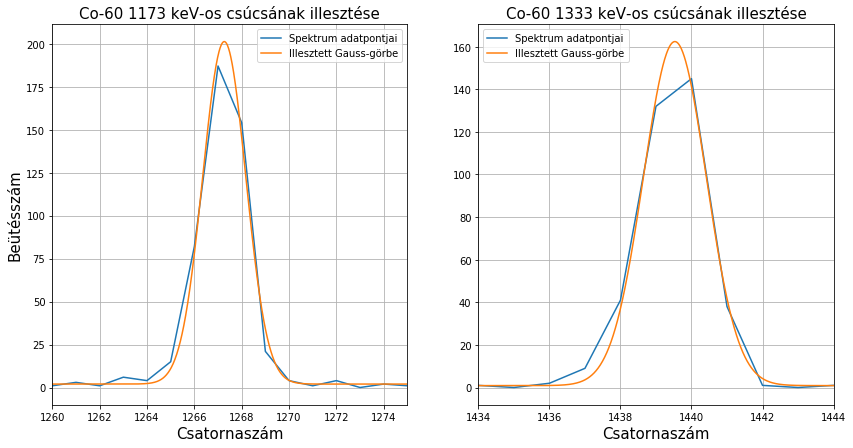
\includegraphics[scale=0.50]{Co_hpg}
\caption{A kobalt első (1173 keV) és második (1333 keV) csúcsának illesztése a HPG-vel felvett spektrum esetén}
\label{fig:8}
\end{figure}

\newpage

Az illesztési paraméterek:

\begin{table}[!h]
\begin{center}
\begin{tabular}{|c|c||c|}
\hline
- & 1173 keV & 1333 keV \\
\hline
$A$ & $199.211 \pm 4.460$ & $161.513 \pm 3.236$ \\
\hline
$\mu$ & $1267.263 \pm 0.023$ & $1439.532 \pm 0.020$ \\ 
\hline
$\sigma$ & $0.909 \pm 0.243$ & $0.886 \pm 0.022$ \\
\hline
$c$ & $2.000 \pm 1.130$ & $0.890 \pm 1.047$ \\
\hline
\end{tabular}
\caption{$^{60}$Co csúcsokra vonatkozó illesztési paraméterek}
\end{center}
\end{table}

A cézium csúcsának illesztése (\ref{fig:9} . ábra):

\begin{figure}[!h]
\centering
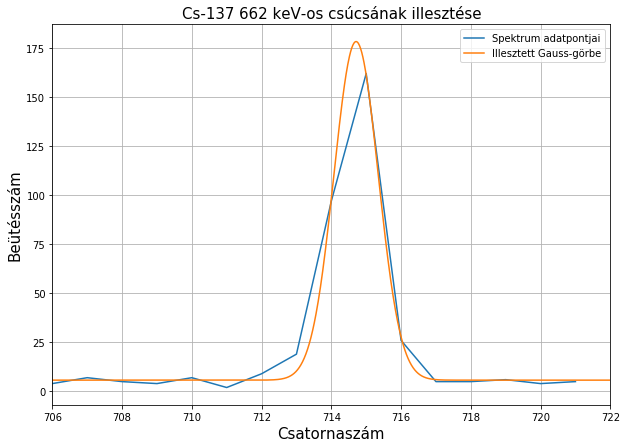
\includegraphics[scale=0.60]{Cs137_1csucs_hpg}
\caption{A cézium csúcsának (662 keV) illesztése}
\label{fig:9}
\end{figure}

Az illesztési paraméterek:
\begin{table}[!h]
\begin{center}
\begin{tabular}{|c|c|}
\hline
Energia & 662 keV \\ 
\hline
$A$ & $172.539 \pm 4.197$\\
\hline
$\mu$ & $714.710 \pm 0.017$\\
\hline
$\sigma$ & $0.636 \pm 0.020$\\
\hline
$c$ & $5.750 \pm 0.894$\\
\hline
\end{tabular}
\caption{A cézium spektrumában látható csúcs illesztési paraméterei}
\end{center}
\end{table}

\newpage

Az illesztési paraméterek segítségével ezen detektor esetében is el tudjuk végezni a kalibrációt, szintén egyenesillesztés segítségével, a fent már kifejtett módon. A kalibrációs egyenes a \ref{fig:10} . ábrán látható.

\begin{figure}[!h]
\centering
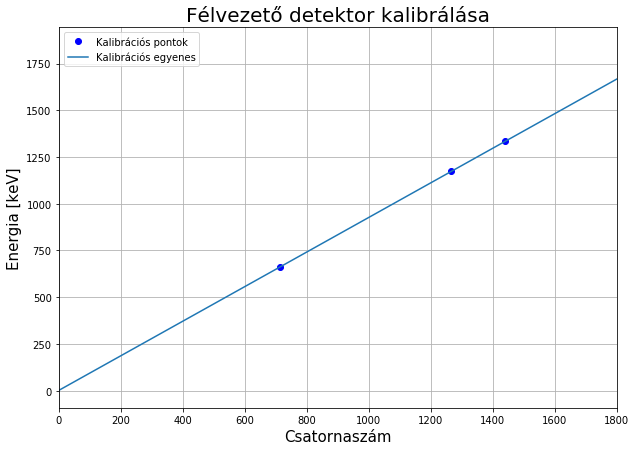
\includegraphics[scale=0.60]{HPG_kalib}
\caption{A félvezető detektor kalibrálásához készített egyenesillesztés}
\label{fig:10}
\end{figure}

A kalibrációs egyenes egyenlete:

$$E(x)=0.926 \cdot x + 0.450$$

A detektor felbontóképességét itt is a $^{60}$Co vonal félértékszélességével írhatjuk le a \ref{fig:4} . ábránál tapasztaltakhoz hasonlóan. Ez alapján a HPG felbontóképességére $\Delta x = (1.935 \pm 0.049)$ keV adódik. Ezen felbontásérték segítségével közelítőleg azonosítani tudunk bizonyos bomlástermékeket a HPG spektrumában. A feladatunk a $^{238}$U három bomlástermékének, a $^{214}$Bi (609.318 keV), $^{214}$Pb (351.9 keV) és a $^{214}$Pb (295.2 keV) csúcsának spektrumon belüli azonosítása volt. Ehhez kivágtuk a spektrum irodalmi energiaérték körüli tartományát, majd a felbontóképességen belül detektálható csúcsot azonosítottuk a keresett leányelemként. A spektrumrészletek és a csúcsok azonosításai a \ref{fig:11} . ábrán látható.
\newpage

\begin{figure}[!h]
\centering
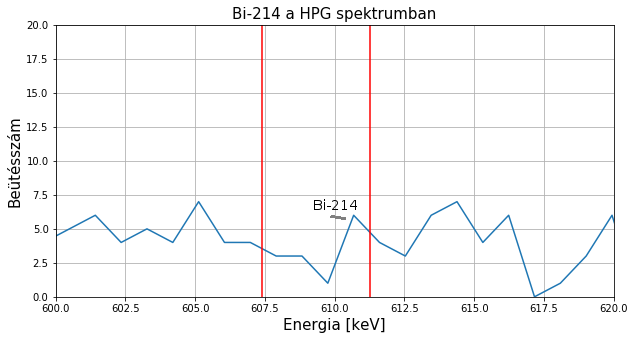
\includegraphics[scale=1]{Bi_csucs}
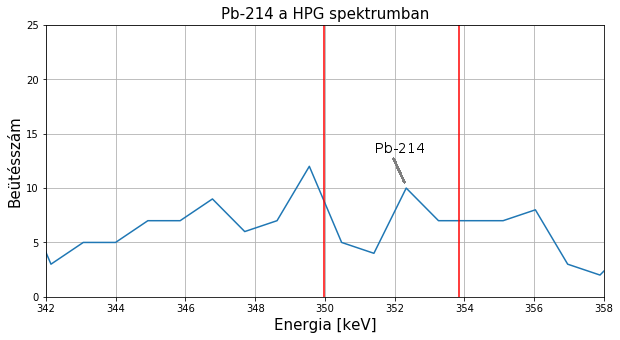
\includegraphics[scale=1]{Pb_csucs}
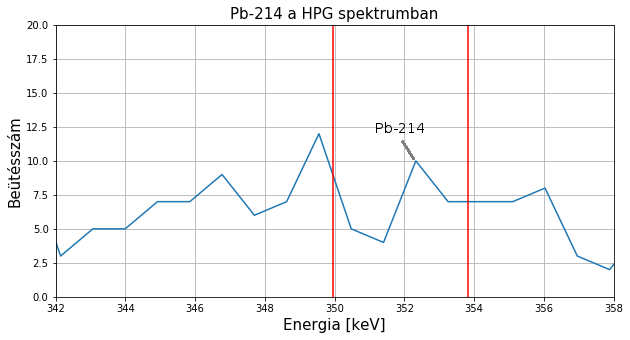
\includegraphics[scale=1]{Pb_2csucs}

\caption{$^{238}$U leányelemeinek azonosítása. A piros sávok a felbontóképességet jelölik, a sávok között félúton az irodalmi energiaértékek helyezkednek el}\label{fig:11}
\end{figure}
\newpage

A választott csúcsok leolvasott energiaértékei az alábbi táblázatban láthatók:
\begin{table}[!h]
\begin{center}
\begin{tabular}{|c|c|c|}
\hline
Izotóp & Irodalmi energia [keV] & Leolvasott energia [keV]\\
\hline
$^{214}$Bi & 609.32 & 610.68\\
\hline
$^{214}$Pb & 351.90 & 352.33\\
\hline
$^{214}$Pb & 295.20 & 296.77\\ 
\hline
\end{tabular}
\caption{A leányelemek leolvasott helyei. A választott csúcsok mind a kontinuum statisztikus ingadozása felett (Poisson-hiba), valamint a felbonthatósági határon belül vannak}
\end{center}
\end{table}

A táblázatban látható irodalmi értékeket a [2]-ból írtam ki. A spektrumokban az ábrákon látható módon fel lehet lelni az urán leányelemei által létrehozott csúcsokat, azonban a pontosabb energiaméréshez és a csúcsok jobban láthatóvá tételéhez hosszabb idejű mérésekre lett volna szükség. 

%\newpage

\section{Béta spektroszkópia}

A $\beta$-spektroszkópiával kapott spektrum ellentétnem a $\gamma$-val spektroszkópia során kapott spektrumtól folytonos karakterisztikájú, mivel itt a bomlás során kelektkező neutrínó is energiát, illetve impulzust vihet el. Ennek következtében a kilépő elektron, illetve pozitron energiája tetszőleges értéket vehet fel. Használjuk a következők során a $c=m_e=1$ egységrendszert. Ekkor a következő összefüggés lesz érvényes:

\begin{equation*}
p^2= W^2 - 1
\end{equation*}

Amely összefüggésben szereplő W a következőnek adódik:

\begin{equation*}
W= \dfrac{E}{m_ec^2} + 1
\end{equation*}

Az egyes energiákon vett intenzitást a következő formula határozza meg:

\begin{equation*}
N^{\pm}(E)= Kp(E+m_ec^2)(E_m-E)^2F^{\pm}(Z,E)S_n(E)
\end{equation*}

A $\pm$ a pozitron, illetve az elektronhoz tartozó függvényt jelöli. Az $E_m$ jelöli az átmenethez tartozó teljes energiát, az E pedig a részecske energiáját jelöli. Az $F^{\pm}(Z,E)$ pedig a Fermi-függvény, amely megadja a Z rendszámú atommag hatását a keletkező részecskén. Ezen felül bevezethető a módosított Fermi-függvény a következő módon: 

\begin{equation*}
G=\frac{p}{W}F(E,Z)
\end{equation*}

Ezen egyenletekből levezethető az alábbi összefüggés: 

\begin{equation*}
Q=\sqrt{\dfrac{N}{GW^2}}=\kappa (W_m-W)\sqrt{S_n}
\end{equation*}

\newpage

\subsection{Kalibráció}

Mérésünkhöz szükség van a műszer kalibrálására, erre ebben a mérésrészben két ismert értéket használunk fel, a $^{137}$Cs keV-nél lévő konverziós elektronból származó csúcsát és műszer 12-es csatorjánál lévő 0-s keV-nek tekintett küszöbszintjét használjuk fel. Ezeket a következő táblázatban foglaljuk össze: 

\begin{table}[h!]
\centering
\begin{tabular}{|c|c|}
\hline
Csatornaszám (cs) & E[keV] \\ \hline
11 & 0 \\ \hline
$85 \pm 1$ & 630 \\ \hline
\end{tabular}
\end{table}

\begin{figure}[!h]
\centering
\includegraphics[scale=0.30]{kalib2.png}
\caption{A $\beta$-spektroszkópia kalibrálásához készített egyenesillesztés}
\label{fig:12}
\end{figure}


Ezekre az adatokra egyenest illesztünk (\ref{fig:12} . ábra), a kapott illesztési paraméterek: 
\begin{equation*}
\begin{split}
m=10.328 \hspace*{5pt} \mathrm{keV/cs}\\ 
b =-123,934 \hspace*{5pt} \mathrm{keV}
\end{split}
\end{equation*}
Az energia meg kifejezhető a következő módon: 

\begin{equation*}
E=m\cdot cs+b
\end{equation*}
\newpage

\subsection{$^{137}$Cs átmentek meghatározása}

\begin{figure}[!h]
\centering
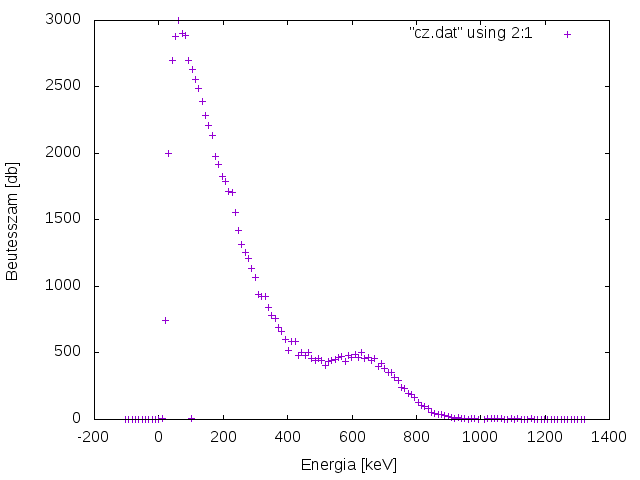
\includegraphics[scale=0.60]{cz.png}
\caption{A $^{137}$Cs N(E) grafikonja}
\label{fig:13}
\end{figure}

Először a beütésszámot ábrázoltuk az energia függvényében (\ref{fig:13} . ábra), majd a Q-t a W függvényében. Ha a transzformált grafikon konverziós csúcs előtti részére egyenest illesztünk (\ref{fig:14} . ábra), akkor az illesztett egyenes paramétereiből meghatározható az $E_m$. 
Az illesztett egyenes paraméterei:

\begin{figure}[!h]
\centering
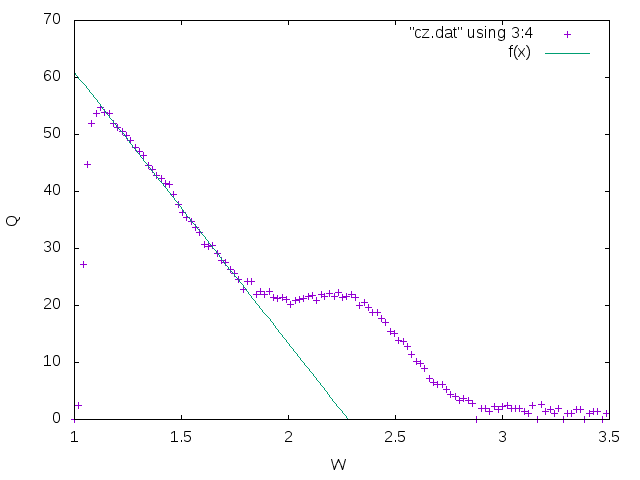
\includegraphics[scale=0.60]{czfit.png}
\caption{A $^{137}$Cs $\sqrt{N}/W(E)$ grafikonja}
\label{fig:14}
\end{figure}
\newpage

\begin{equation*}
\begin{split}
m = -47.600 \pm 0.570\\
b = 108.518 \pm 0.813
\end{split}
\end{equation*}

Ebből következik: 

\begin{equation*}
W_m = - \dfrac{b}{a} = 2.279 \pm 0.071
\end{equation*}

Innen meghatározható a $^{137}$Cs-hoz tartozó maximális energia: $$E_{m} = 653 \pm 35\hspace*{5pt}  \mathrm{keV}.$$.

\subsection{$^{90}$Sr átmeneteinek meghatározása}

\begin{figure}[!h]
\centering
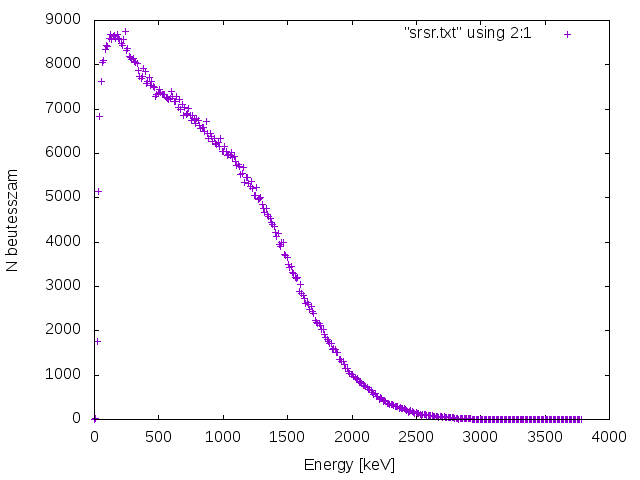
\includegraphics[scale=0.60]{srout.png}
\caption{A $^{90}$Sr N(E) grafikonja}
\label{fig:15}
\end{figure}

A stroncium esetében két párhuzamos $\beta$-bomlás zajlik, emiatt ezek az együttes spektrumát látjuk, így ezekhez külön részletekben (\ref{fig:16} . és \ref{fig:17} . ábra) határoztuk meg a maximális energiákat az előző fejezetben említett módon. 
\newpage
\begin{figure}[!h]
\centering
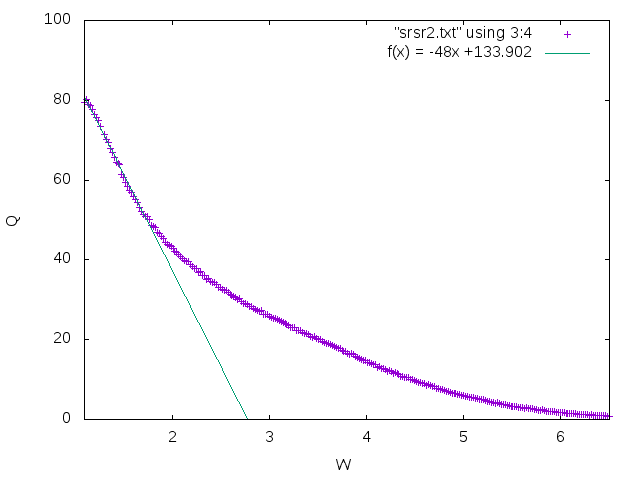
\includegraphics[scale=0.60]{srfit.png}
\caption{A $^{90}$Sr $\sqrt{N}/W(E)$ grafikonja}
\label{fig:16}
\end{figure}

Az első esetben az illesztett egyenes paraméterei:

\begin{equation*}
\begin{split}
m =-48.235 \pm 0.744\\
b = 133.960 \pm 1.126
\end{split}   
\end{equation*}

Ebből az energia maximuma a következő lesz: $$E_{m;1} = 915 \pm 50\hspace*{5pt} \mathrm{keV}$$
%\newpage
\begin{figure}[!h]
\centering
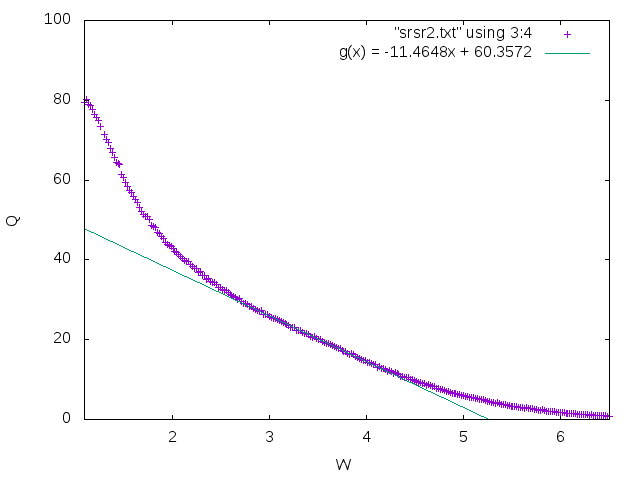
\includegraphics[scale=0.60]{srfit2.png}
\caption{A $^{90}$Sr $\sqrt{N}/W(E)$ grafikonja}
\label{fig:17}
\end{figure}
\newpage
A másik esetben pedig az illesztett paraméterek a következők lesznek: 

\begin{equation*}
\begin{split}
m = -11.465 \pm 0.054\\
b = 60.357 \pm 0.184
\end{split}   
\end{equation*}

Ebből az energia maximumának értéke a következő lesz: $$E_{m;2} = 2179 \pm 41\hspace*{5pt} \mathrm{keV}$$.
\subsection{Háttér}

Végeztünk egy hosszabb mérést (10 órás) a háttéren. Ennek a grafikonja\\ (\ref{fig:18} . ábra) a következő módon néz ki:

\begin{figure}[!h]
\centering
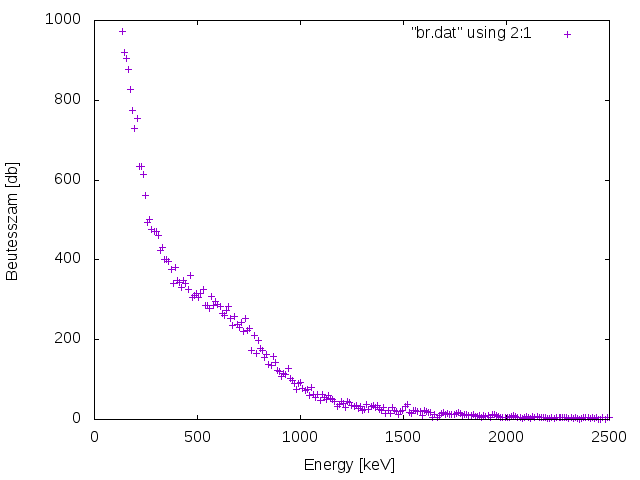
\includegraphics[scale=0.60]{hatter.png}
\caption{A háttér N(E) grafikonja}
\label{fig:18}
\end{figure}
Arra a következtetésre jutottam, hogy a hátteret nem szükséges levonni, mert a statisztikus hiba által okozott eltérés mellett a háttér elhanyagolható, a mérés pontosságát illetően a levonása nem okozna szignifikáns javulást.


\newpage

\section{Diszkusszió}
A mérési feladatokat sikeresen elvégeztük, a mérés, illetve a kiértékelés során kapott eredmények az alábbiakban láthatók. Az eredményeket a [3] honlapon lévő feladatok kitűzésével azonos sorrendben ismertetem.\newline
\subsection{Szcintillációs gamma kalibrációs paraméterek:}
\begin{itemize}
\item $^{60}$Co:
\begin{center}
\begin{tabular}{|c|c||c|}
\hline
Energia & 1173 keV & 1333 keV \\ 
\hline
$A$ & $115.619 \pm 18.067$ & $57.927 \pm 11.078$\\
\hline
$\mu$ & $160.286 \pm 0.400$ & $181.849 \pm 0.171$\\
\hline
\end{tabular}
\end{center}
\item $^{137}$Cs:
\begin{center}

\begin{tabular}{|c|c|}
\hline
Energia & 662 keV \\ 
\hline
$A$ & $547.931 \pm 8.419$\\
\hline
$\mu$ & $92.557 \pm 0.076$\\
\hline
\end{tabular}
\end{center}
\item A kalibráció egyenes egyenlete:
\begin{equation*}
E(x)=7.522x-33.903
\end{equation*}
\end{itemize}
\subsection{Detektor felbontása}
\begin{equation*}
\Delta x=(10.934 \pm 2.475)\mathrm{keV}
\end{equation*}
\subsection{NaCl és KCl-al mért K-40 intenzitás arányok}
\begin{center}
0.092 $\pm$ 0.012
\end{center}
\subsection{HPG gamma kalibrációs paraméterek}
\begin{itemize}
\item $^{60}$Co:
\begin{center}
\begin{tabular}{|c|c||c|}
\hline
Energia & 1173 keV & 1333 keV \\ 
\hline
$A$ & $199.211 \pm 4.46$ & $161.513 \pm 3.236$\\
\hline
$\mu$ & $1267.263 \pm 0.023$ & $1439.532 \pm 0.02$\\
\hline
\end{tabular}
\end{center}
\item $^{137}$Cs:
\begin{center}

\begin{tabular}{|c|c|}
\hline
Energia & 662 keV \\ 
\hline
$A$ & $172.539 \pm 4.197$\\
\hline
$\mu$ & $714.71 \pm 0.017$\\
\hline
\end{tabular}
\end{center}
\item Kalibrációs egyenes egyenlete:
\begin{equation*}
E(x)=0.926x +0.45
\end{equation*}
\end{itemize}
\subsection{HPG felbontóképessége}
\begin{equation*}
\Delta x=(1.935 \pm 0.45)\mathrm{keV}
\end{equation*}
Összehasonlítva ezt a fenti, szcintillációs detektor felbontására kapott értékkel látszik, hogy a HPG-nek körülbelül 10-szer jobb a felbontása.
\subsection{U-238 leányelemek azonosítása}
\begin{center}
\begin{tabular}{|c|c|c|}
\hline
$^{214}$Bi & 609.32 & 610.68\\
\hline
$^{214}$Pb & 351.90 & 352.33\\
\hline
$^{214}$Pb & 295.20 & 296.77\\ 
\hline
\end{tabular}
\end{center}
\subsection{Béta szcintillációs kalibrációs egyenes egyenlete}
\begin{equation*}
E=(10.3279\cdot cs -123.934) keV
\end{equation*}
\subsection{$^{137}$Cs átmenetek}
\begin{itemize}
\item{Illesztett egyenes paraméterei:
\begin{equation*}
\begin{split}
m=-47.600\pm 0.570\\
b=108.518 \pm 0.813
\end{split}
\end{equation*}
}
\item{$W_m=2.279\pm0.071$}
\item{$E_m=653\pm 35$ keV}
\end{itemize}
\subsection{$^{90}$Sr átmenetek (1. bomlás)}
\begin{itemize}
\item{Illesztett egyenes paraméterei:
\begin{equation*}
\begin{split}
m=-48.235\pm 0.744\\
b=133.960 \pm 1.126
\end{split}
\end{equation*}
}
\item{$E_m=915\pm 50$ keV}
\end{itemize}
\subsection{$^{90}$Sr átmenetek (2. bomlás)}
\begin{itemize}
\item{Illesztett egyenes paraméterei:
\begin{equation*}
\begin{split}
m=-11.465\pm 0.054\\
b=60.357 \pm 0.184
\end{split}
\end{equation*}
}
\item{$E_m=2179\pm 41$ keV}
\end{itemize}

\section*{Hivatkozások}
\hspace*{14pt} [1] : \emph{Félértékszélesség meghatározása}:\\
\hspace*{34pt} \texttt{http://atomfizika.elte.hu/muszerek/MSP/felertek.pdf}\\

[2] : \emph{Urán leányelemeinek adatai}:\\
\hspace*{34pt} \texttt{http://atomfizika.elte.hu/muszerek/MSP/Uran\_torium\_sor.png}\\

[3] : \emph{Mérési feladatok}:\\
\hspace*{34pt} \texttt{http://atomfizika.elte.hu/muszerek/MSP/MSP\_pontok.php}
\end{document}